\documentclass{beamer}
\usepackage[utf8]{inputenc}
\usepackage[english]{babel}

% -- Including some standard packages --
\usepackage{graphicx}
\usepackage{soul}
\usepackage{hyperref}
\usepackage{colortbl}
\usepackage{dsfont}
\usepackage{soul}

% -- Choosing theme --

\usetheme{Boadilla}
\usecolortheme{whale}
\setbeamercolor{alerted text}{fg=purple} % Making alerted text non-red

% Tikz
\usepackage{tikz}
\usetikzlibrary{matrix,positioning,fit,backgrounds,intersections}

% -- Cross signs --
\usepackage{pifont} % http://ctan.org/pkg/pifont
\newcommand{\cmark}{\ding{51}}%
\newcommand{\xmark}{\ding{55}}%
\newcommand{\xopt}{\ding{48}}%

% -- Custom commands --
\DeclareMathOperator*{\argmax}{arg\,max}
\DeclareMathOperator*{\argmin}{arg\,min}

\title[Mathematics II]{\textbf{Mathematics for Cryptography II: Security Analysis, Polynomials, Number Theory}}
\author{Distributed Lab}
\date{July 18, 2024}
\titlegraphic{
    
\includegraphics[width=\textwidth]{images/banner_wide.png}
}

\expandafter\def\expandafter\insertshorttitle\expandafter{%
  \insertshorttitle\hfill%
  \insertframenumber\,/\,\inserttotalframenumber}

\AtBeginSection[]{
  \begin{frame}
  \vfill
  \centering
  \begin{beamercolorbox}[sep=8pt,center,shadow=true,rounded=true]{title}
    \usebeamerfont{title}\insertsectionhead\par%
  \end{beamercolorbox}
  \vfill
  \end{frame}
}

\begin{document}
    \frame {
      \titlepage
    }
  
    \begin{frame}{Plan}
      \tableofcontents
    \end{frame}

    \begin{frame}{What will we learn today?}
        How to read\ldots This\ldots

        \begin{figure}
            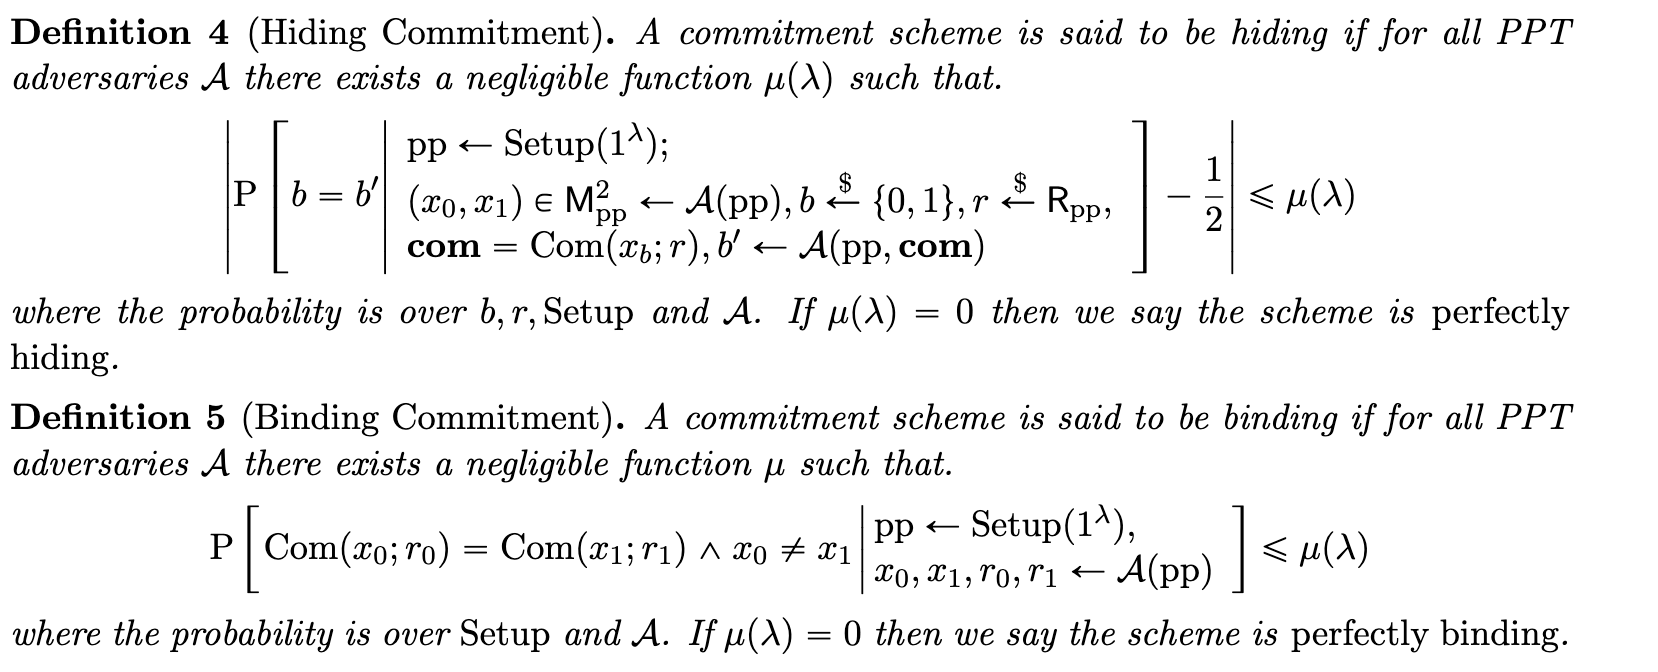
\includegraphics[width=0.8\textwidth]{images/lecture_2/bulletproof.png}
            \caption{This is not that hard as it seems. Figure from ``\textit{Bulletproofs: Short Proofs for Confidential Transactions and More}''}
            \label{fig:wuuttt}
          \end{figure}
    \end{frame}

    \section{Quick Recap}

    \begin{frame}{Quick Recap}
        \begin{enumerate}
            \item We know how to read formal statements, like 
            \begin{equation}
                (\forall n \in \mathbb{N}) \, (\exists k \in \mathbb{Z}): \{n=2k+1 \vee n = 2k\}
            \end{equation}
            \item Group $\mathbb{G}$ is a set with a binary operation that satisfies certain rules. In this lecture, we will use the \textbf{multiplicative} notation: for example, $g^{\alpha}$ means $g$ multiplied by itself $\alpha$ times.
            \item Probability of event $E$ is denoted by $\text{Pr}[E]$ -- we will need it further.
        \end{enumerate}
    \end{frame}

    \section{Polynomials}

    \subsection{Definition}

    \begin{frame}{Definition}
      \begin{definition}
        A \textbf{polynomial} $f(x)$ is a function of the form
        \begin{equation*}
            p(x) = c_0 + c_1 x + c_2 x^2 + \cdots + c_n x^n = \sum_{k=0}^{n} c_k x^k,
        \end{equation*}
        where $c_0, c_1, \dots, c_n$ are coefficients of the polynomial.
    \end{definition}
    
    \begin{definition}
        A set of polynomials depending on $x$ with coefficients in a field $\mathbb{F}$ is denoted as $\mathbb{F}[x]$, that is
        \begin{equation*}
            \mathbb{F}[x] = \left\{p(x) = \sum_{k=0}^{n} c_k x^k: c_k \in \mathbb{F}, \; k = 0,\dots,n\right\}.
        \end{equation*}
    \end{definition}
    \end{frame}

    \begin{frame}{Examples of Polynomials}
      \begin{example}
        Consider the finite field $\mathbb{F}_3$. Then, some examples of polynomials from $\mathbb{F}_3[x]$ are listed below:
        \begin{enumerate}
            \item $p(x) = 1 + x + 2x^2$.
            \item $q(x) = 1 + x^2 + x^3$.
            \item $r(x) = 2x^3$.
        \end{enumerate}
    
       If we were to evaluate these polynomials at $1 \in \mathbb{F}_3$, we would get:
        \begin{enumerate}
            \item $p(1) = 1 + 1 + 2 \cdot 1 \; \text{mod} \; 3 = 1$.
            \item $q(1) = 1 + 1 + 1 \; \text{mod} \; 3 = 0$.
            \item $r(1) = 2 \cdot 1 = 2$.
        \end{enumerate}
    \end{example}
    \end{frame}    

    \begin{frame}{More about polynomials}
      \begin{definition}
          The \textbf{degree} of a polynomial $p(x) = c_0+c_1x+c_2x^2+\dots$ is the largest $k \in \mathbb{Z}_{\geq 0}$ such that $c_k \neq 0$. We denote the degree of a polynomial as $\deg p$. We also denote by $\mathbb{F}^{(\leq m)}[x]$ a set of polynomials of degree at most $m$.
      \end{definition}
      
      \begin{example}
          The degree of the polynomial $p(x) = 1 + 2x + 3x^2$ is $2$, so $p(x) \in \mathbb{F}_3^{(\leq 2)}[x]$.
      \end{example}
      
      \begin{theorem}
          For any two polynomials $p,q \in \mathbb{F}[x]$ and $n = \deg p, m = \deg q$, the following two statements are true:
          \begin{enumerate}
              \item $\deg (pq) = n + m$.
              \item $\deg (p + q) = \max\{n,m\}$ if $n \neq m$ and $\deg (p+q) \leq m$ for $m=n$.
          \end{enumerate}
      \end{theorem}
    \end{frame}
    \subsection{Roots and Divisibility}
    \begin{frame}{Roots of Polynomials}
      \begin{definition}
          Let $p(x) \in \mathbb{F}[x]$ be a polynomial of degree $\deg p \geq 1$. A field element $x_0 \in \mathbb{F}$ is called a root of $p(x)$ if $p(x_0) = 0$.
      \end{definition}
      
      \begin{example}
          Consider the polynomial $p(x) = 1 + x + x^2 \in \mathbb{F}_3[x]$. Then, $x_0=1$ is a root of $p(x)$ since $p(x_0) = 1 + 1 + 1 \; \text{mod} \; 3 = 0$.
      \end{example}

      \begin{theorem}
        Let $p(x) \in \mathbb{F}[x], \deg p \geq 1$. Then, $x_0 \in \mathbb{F}$ is a root of $p(x)$ if and only if there exists a polynomial $q(x)$ (with $\deg q = n-1$) such that
        \begin{equation*}
            p(x) = (x-x_0)q(x)
        \end{equation*}
    \end{theorem}
    \end{frame}
    \begin{frame}{Polynomial Division}
      \begin{theorem}
        Given $f,g \in \mathbb{F}[x]$ with $g \neq 0$, there are unique polynomials $p,q \in \mathbb{F}[x]$ such that 
        \begin{equation*}
            f = q \cdot g + r, \; 0 \leq \deg r < \deg g
        \end{equation*}
    \end{theorem}
    
    \begin{example}
        Consider $f(x) = x^3+2$ and $g(x) = x+1$ over $\mathbb{R}$. Then, we can write $f(x) = (x^2-x+1)g(x) + 1$, so the remainder of the division is $r \equiv 1$. Typically, we denote this as:
        \begin{equation*}
            f \, \text{div} \, g = x^2-x+1, \quad f \, \text{mod} \, g = 1.
        \end{equation*}
    
        The notation is pretty similar to one used in integer division.
    \end{example}
    \end{frame}

    \begin{frame}{Polynomial Divisibility}
      \begin{definition}
        A polynomial $f(x) \in \mathbb{F}[x]$ is called \textbf{divisible} by $g(x) \in \mathbb{F}[x]$ (or, $g$ \textbf{divides} $f$, written as $g \mid f$) if there exists a polynomial $h(x) \in \mathbb{F}[x]$ such that $f=gh$.
    \end{definition}
    
    \begin{theorem}
        If $x_0 \in \mathbb{F}$ is a root of $p(x) \in \mathbb{F}[x]$, then $(x-x_0) \mid p(x)$.
    \end{theorem}
    
    \begin{definition}
        A polynomial $f(x) \in \mathbb{F}[x]$ is said to be \textbf{irreducible} in $\mathbb{F}$ if there are no polynomials $g,h \in \mathbb{F}[x]$ both of degree more than $1$ such that $f = gh$.
    \end{definition}
    \end{frame}

    \begin{frame}{Polynomial Divisibility}
      \begin{example}
        A polynomial $f(x) = x^2+16$ is irreducible in $\mathbb{R}$. Also $f(x) = x^2-2$ is irreducible over $\mathbb{Q}$, yet it is reducible over $\mathbb{R}$: $f(x) = (x-\sqrt{2})(x+\sqrt{2})$. 
    \end{example}
    
    \begin{example}
        There are no polynomials over complex numbers $\mathbb{C}$ with degree more than $2$ that are irreducible. This follows from the \textit{fundamental theorem of algebra}. For example, $x^2+16 = (x-4i)(x+4i)$.
    \end{example}
    \end{frame}
    \subsection{Interpolation}
    \begin{frame}{Interpolation}
      \begin{alertblock}{Question}
        How can we define the polynomial?
      \end{alertblock}

      The most obvious way is to specify coefficients $(c_0,c_1,\dots,c_n)$. Can we do it in a different way?

      \begin{theorem}
        Given $n+1$ distinct points $(x_0,y_0),\dots,(x_n,y_n)$, there exists a unique polynomial $p(x)$ of degree at most $n$ such that $p(x_i) = y_i$ for all $i=0,\dots,n$.
      \end{theorem}
    \end{frame}

    \begin{frame}{Illustration with two points}
      \begin{figure}
        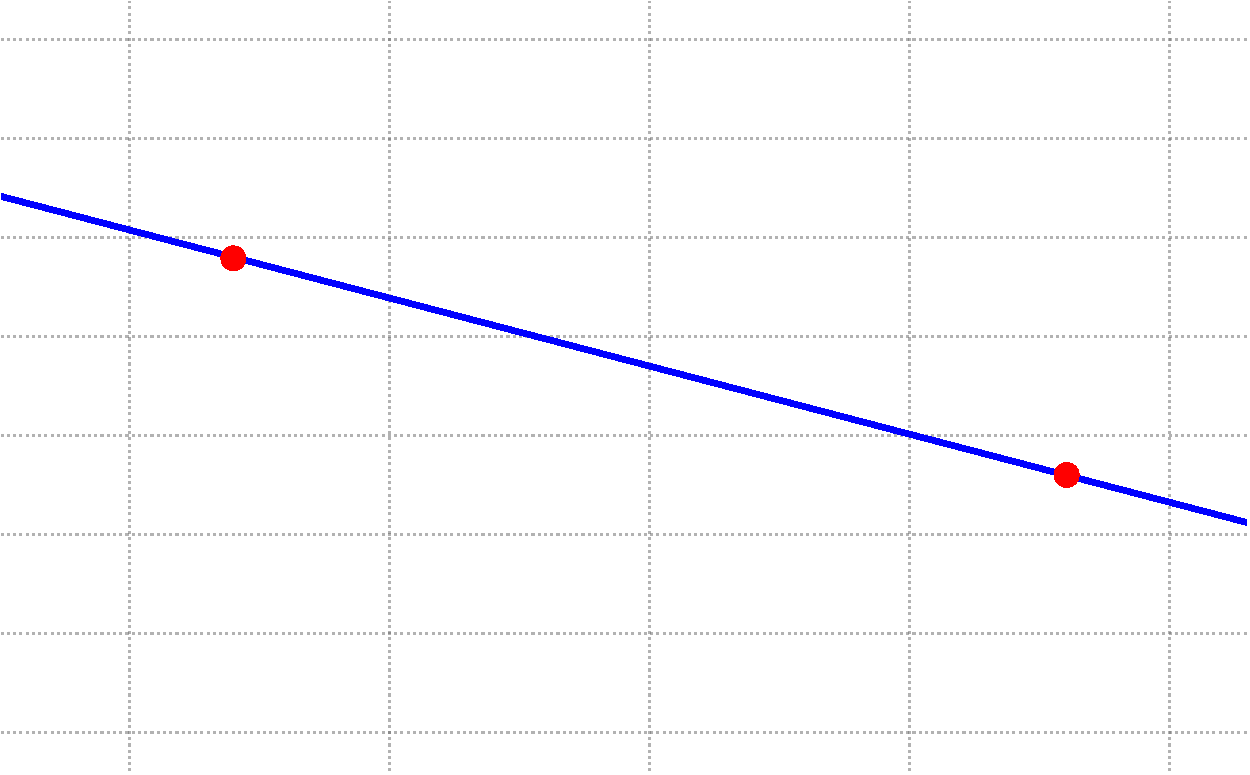
\includegraphics[width=0.8\textwidth]{images/lecture_1/simple_interpolation.pdf}
        \caption{$2$ points on the plane uniquely define the polynomial of degree $1$ (linear function).}
        \label{fig:simple_interpolation}
      \end{figure}
    \end{frame}

    \begin{frame}{Illustration with five points}
      \begin{figure}
        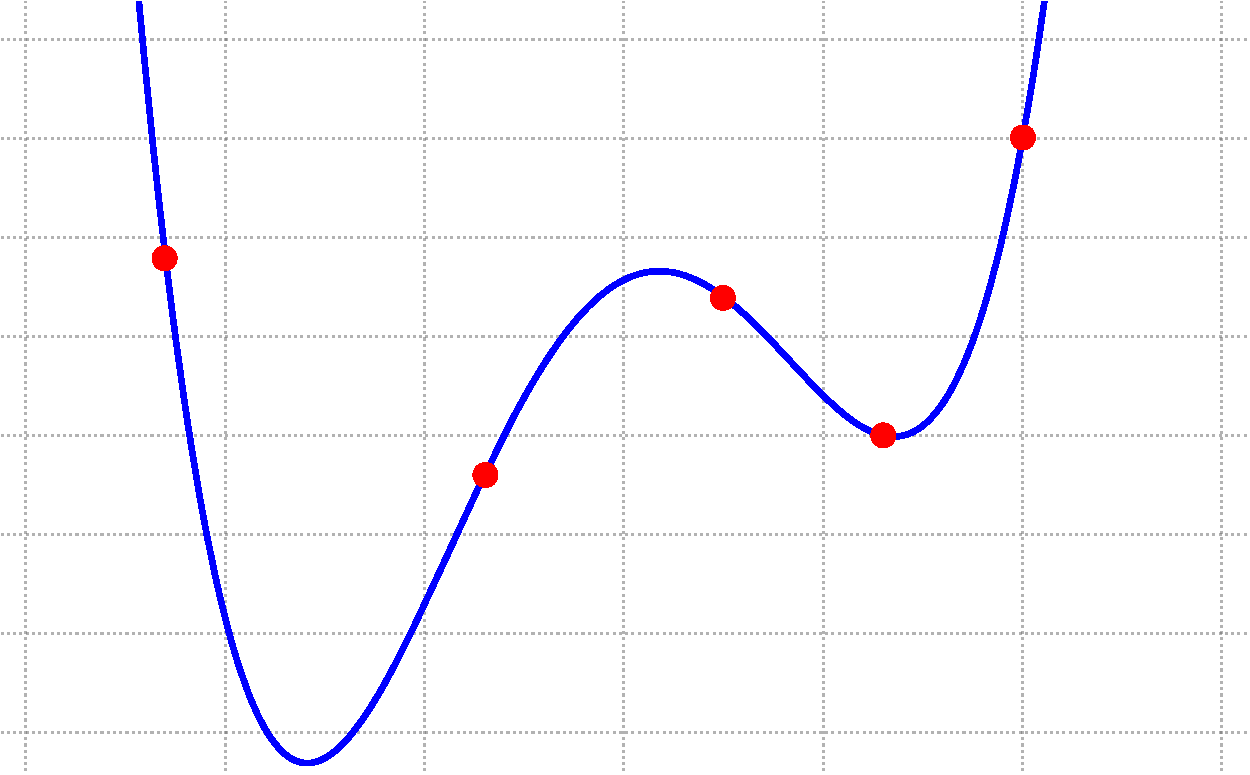
\includegraphics[width=0.8\textwidth]{images/lecture_1/interpolation.pdf}
        \caption{$5$ points on the plane uniquely define the polynomial of degree $4$.}
        \label{fig:interpolation}
      \end{figure}
    \end{frame}

    \begin{frame}{Illustration with three points}
      \begin{figure}
        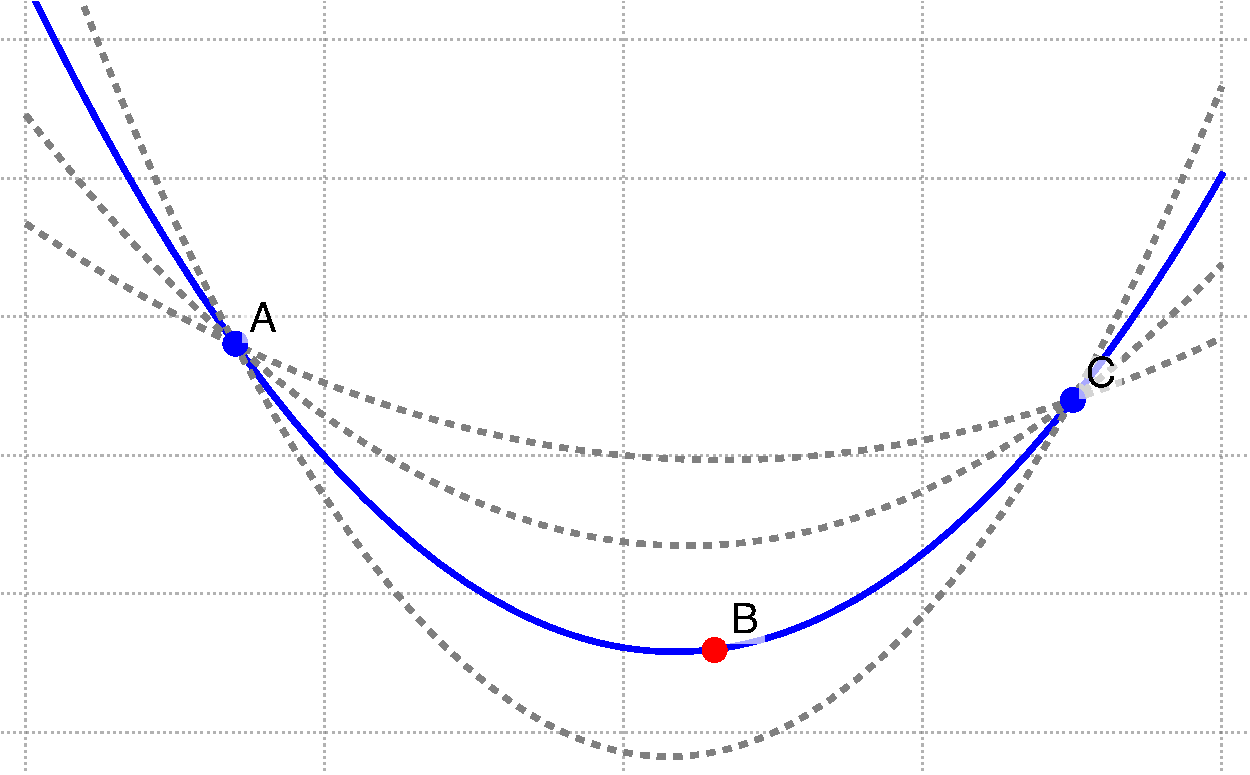
\includegraphics[width=0.8\textwidth]{images/lecture_1/shamir_demo.pdf}
        \caption{$2$ points are not enough to define the quadratic polynomial ($c_2x^2+c_1x+c_0$).}
        \label{fig:interpolation}
      \end{figure}
    \end{frame}

    \begin{frame}{Lagrange Interpolation}
      One of the ways to interpolate the polynomial is to use the Lagrange interpolation.

      \begin{theorem}
        Given $n+1$ distinct points $(x_0,y_0),\dots,(x_n,y_n)$, the polynomial $p(x)$ that passes through these points is given by
        \begin{equation*}
            p(x) = \sum_{i=0}^{n} y_i \ell_i(x), \quad \ell_i(x) = \prod_{i=0, j \neq i}^n \frac{x-x_j}{x_i-x_j}.
        \end{equation*}
    \end{theorem}
    \end{frame}

    \subsection{Interpolation Applications: Shamir Secret Sharing}
    \begin{frame}{Application: Shamir Secret Sharing}
      \begin{alertblock}{Motivation}    
        How to share a secret $\alpha$ among $n$ people in such a way that any $t$ of them can reconstruct the secret, but any $t-1$ cannot?
      \end{alertblock}  

      \begin{definition}
        \textbf{Secret Sharing} scheme is a pair of efficient algorithms $(\mathsf{Gen}, \mathsf{Comb})$ which work as follows:
        \begin{itemize}
            \item $\mathsf{Gen}(\alpha, t, n)$: probabilistic sharing algorithm that yields $n$ shards $(\alpha_1,\dots,\alpha_t)$ for which $t$ shards are needed to reconstruct the secret $\alpha$.
            \item $\mathsf{Comb}(\mathcal{I}, \{\alpha_i\}_{i \in \mathcal{I}})$: deterministic reconstruction algorithm that reconstructs the secret $\alpha$ from the shards $\mathcal{I} \subset \{1,\dots,n\}$ of size $t$.
        \end{itemize}
    \end{definition}
    \end{frame}

    \begin{frame}{Shamir's Protocol}
      \begin{block}{Note}
        Here, we require the \textbf{correctness}: for every $\alpha \in F$, for every possible output $(\alpha_1,\dots,\alpha_n) \gets \mathsf{Gen}(\alpha, t, n)$, and any $t$-size subset $\mathcal{I}$ of $\{1,\dots,n\}$ we have
        \begin{equation}
            \mathsf{Comb}(\mathcal{I}, \{\alpha_i\}_{i \in \mathcal{I}}) = \alpha.
        \end{equation}
      \end{block}

      \begin{definition}
        Now, \textbf{Shamir's protocol} works as follows: $F=\mathbb{F}_q$ and
        \begin{itemize}
            \item $\mathsf{Gen}(\alpha, k, n)$: choose random $k_1,\dots,k_{t-1} \xleftarrow[]{R} \mathbb{F}_q$ and define the polynomial
            \begin{equation}
                \omega(x) := \alpha + k_1x + k_2x^2 + \cdots + k_{t-1}x^{t-1} \in \mathbb{F}_q^{\leq (t-1)}[x],     
            \end{equation}
            and then compute $\alpha_i \gets \omega(i) \in \mathbb{F}_q, \; i = 1,\dots,n$. 
        \end{itemize}
      \end{definition}
    \end{frame}
  
    \begin{frame}{Shamir's Protocol}
      \begin{definition}
        \begin{itemize}
            \item $\mathsf{Comb}(\mathcal{I}, \{\alpha_i\}_{i \in \mathcal{I}})$: interpolate the polynomial $\omega(x)$ using the Lagrange interpolation and output $\omega(0) = \alpha$.
        \end{itemize}
      \end{definition}

      \begin{figure}
        \centering
        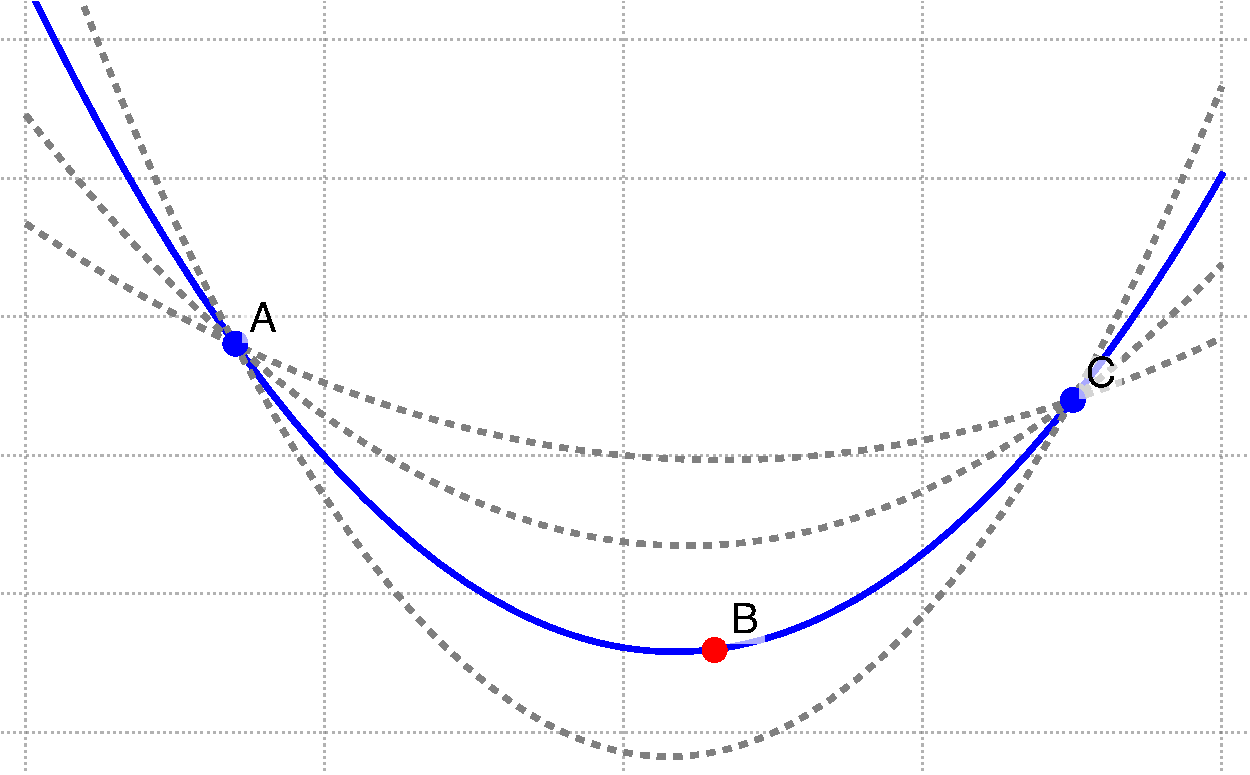
\includegraphics[width=0.5\textwidth]{images/lecture_1/shamir_demo.pdf}
        \caption{There are infinitely many quadratic polynomials passing through two \textcolor{blue}{blue} points (\textcolor{gray}{gray dashed} lines). However, knowing the \textcolor{red}{red} point allows us to uniquely determine the polynomial and thus get its value at $0$.}
        \label{fig:shamir}
      \end{figure}
    \end{frame}
  
    \begin{frame}{}
        \centering \Large
        \emph{Thanks for your attention!}
      \end{frame}
\end{document}